\documentclass[UTF8]{beamer}
\usepackage{ctex} % 支持中文
\usepackage{amsmath}
\usepackage{amssymb} % For symbols like \mathbb{E}, \lim, \sum
\usepackage{graphicx} % For \includegraphics

% --- Theme and Appearance ---
\usetheme{Madrid}
\usecolortheme{default}

\setbeamertemplate{navigation symbols}{}

% --- Custom Colors for Beamer Blocks ---
\setbeamercolor{block title}{bg=blue!20!white, fg=black}
\setbeamercolor{block body}{bg=blue!5!white, fg=black}
\setbeamercolor{example title}{bg=green!20!white, fg=black}
\setbeamercolor{example body}{bg=green!5!white, fg=black}
\setbeamercolor{alertblock title}{bg=red!20!white, fg=black}
\setbeamercolor{alertblock body}{bg=red!5!white, fg=black}

% --- Define math operators for better typography ---
\DeclareMathOperator{\E}{\operatorname{E}}
\DeclareMathOperator{\Var}{\operatorname{Var}}
\DeclareMathOperator{\Prob}{\operatorname{P}}

\title{第七讲 大数定律}
\subtitle{正态分布的普遍性与柯西分布的特殊性} % New subtitle to reflect the focus
\author{龚鹤扬}
\institute{中国科学技术大学统计学博士 \\ 上海芯梯科技有限公司}
\date{\today}

\begin{document}

\begin{frame}
    \titlepage
\end{frame}

\begin{frame}{目录}
    \tableofcontents
\end{frame}

\section{引言}
\begin{frame}[shrink=10]{引言:大数定律的重要性与适用性}
    \framesubtitle{随机现象中的规律性}
    \begin{itemize}
        \item 本讲讨论概率论中一组重要的极限定理——\alert{大数定律 (Law of Large Numbers, LLN)}。
        \item 核心思想:在大量重复试验中,事件发生的\alert{频率}近似于其\alert{概率},样本均值收敛于总体\alert{期望}。
        \item 大数定律是连接\alert{理论概率}与\alert{统计推断}的桥梁。
        \item \alert{重要前提}:大数定律的结论依赖于随机变量满足特定的\alert{条件}(如期望存在、方差有限等)。
        \item 我们将以常见的\alert{正态分布}为例,说明大数定律如何在其条件下成立;并以\alert{柯西分布}为例,探讨当条件不满足时,大数定律为何失效。
    \end{itemize}
\end{frame}

\section{切比雪夫不等式}
\begin{frame}[shrink=5]{7.1 切比雪夫不等式 (Chebyshev's Inequality)}
    \framesubtitle{一个普适的概率上界}
    \begin{itemize}
        \item 切比雪夫不等式给出了随机变量偏离其期望值的概率的一个\alert{上界}。
        \item 这个界不依赖于随机变量的具体分布形式,只需要其\alert{期望}和\alert{方差}存在且有限。
    \end{itemize}
    \pause
    \begin{block}{定理 7.1 (切比雪夫不等式)}
        设随机变量 X 具有期望 $\E(X) = \mu$ 和方差 $\Var(X) = \sigma^2$ (其中 $0 < \sigma^2 < +\infty$)。
        则对于任意正数 $\epsilon > 0$,有:
        \[ \Prob(|X - \mu| \geq \epsilon) \leq \frac{\sigma^2}{\epsilon^2} \]
    \end{block}
    \pause
    \textbf{示例:正态分布}
    \begin{itemize}
        \item 对于正态分布 $N(\mu, \sigma^2)$,其期望为 $\mu$,方差为 $\sigma^2$ (\alert{均存在且有限})。
        \item 因此,切比雪夫不等式适用于正态分布,为 $|X-\mu|$ 的偏离提供了一个(尽管可能宽松的)概率上界。
    \end{itemize}
\end{frame}

\section{弱大数定律 (WLLN)}
\begin{frame}[shrink=5]{7.2 弱大数定律 (WLLN): 切比雪夫方法}
    \framesubtitle{基于方差存在的依概率收敛}
    \begin{block}{定理 7.2 (切比雪夫弱大数定律)}
        设 $X_1, X_2, \dots, X_n, \dots$ 是一列\alert{相互独立}、具有相同期望 $\E(X_i) = \mu$ 和相同\alert{有限方差} $\Var(X_i) = \sigma^2 < +\infty$ 的随机变量序列。
        令样本均值为 $\bar{X}_n = \frac{1}{n} \sum_{i=1}^{n} X_i$。
        则对于任意 $\epsilon > 0$,有:
        \[ \lim_{n \to \infty} \Prob(|\bar{X}_n - \mu| \geq \epsilon) = 0 \quad (\text{即 } \bar{X}_n \xrightarrow{P} \mu) \]
    \end{block}
    \pause
    \textbf{示例:正态分布序列}
    \begin{itemize}
        \item 若 $X_i \sim N(\mu, \sigma^2)$ 且相互独立,则它们满足切比雪夫WLLN的\alert{所有条件} (独立、同期望 $\mu$、同有限方差 $\sigma^2$)。
        \item 因此,i.i.d. 正态随机变量的样本均值 $\bar{X}_n$ \alert{依概率收敛}于总体期望 $\mu$。
    \end{itemize}
    \footnotesize
    \textit{注:此定理依赖于方差存在且有限,并通过切比雪夫不等式证明。}
\end{frame}

\begin{frame}{伯努利弱大数定律}
    \framesubtitle{频率的稳定性}
    \begin{block}{定理 7.3 (伯努利弱大数定律)}
        设 $n_A$ 是 $n$ 次独立重复伯努利试验中事件 A 发生的次数,$p$ 是事件 A 在每次试验中发生的概率。
        令 $f_n = \frac{n_A}{n}$ 为事件 A 发生的频率。
        则对于任意 $\epsilon > 0$: $\lim_{n \to \infty} \Prob\left(\left| f_n - p \right| \geq \epsilon\right) = 0$。
    \end{block}
    \textit{注:这是切比雪夫WLLN的特例,因为伯努利变量 $X_i \sim B(1,p)$ 的 $\E(X_i)=p$ 且 $\Var(X_i)=p(1-p)$ 有限。}
\end{frame}

\begin{frame}[shrink=10]{大数定律的边界:引入柯西分布}
    \framesubtitle{当期望不再可靠}
    \begin{itemize}
        \item 切比雪夫WLLN要求\alert{方差有限}。许多其他版本的大数定律(如辛钦WLLN,柯尔莫哥洛夫SLLN)放宽了对方差的要求,但一个更核心的条件是:\alert{期望的存在性}。
        \pause
        \item \textbf{思考}:如果一个分布连期望都没有,样本均值会收敛到哪里呢?
        \item \alert{柯西分布 (Cauchy Distribution)} 就是这样一个期望不存在的著名例子。
    \end{itemize}
    \pause
    \begin{block}{柯西分布 $C(x_0, \gamma)$}
        PDF: $f(x; x_0, \gamma) = \frac{1}{\pi\gamma [1 + ((x-x_0)/\gamma)^2]}$
        \begin{itemize}
            \item $x_0$: 位置参数 (中位数), $\gamma$: 尺度参数。
            \item 标准柯西 $C(0,1)$ ($x_0=0, \gamma=1$): $f(x) = \frac{1}{\pi (1+x^2)}$。
            \item 特点:重尾,\alert{期望 $\E(X)$ 不存在},\alert{方差 $\Var(X)$ 无限大}。
        \end{itemize}
    \end{block}
    \pause
    \textit{这意味着柯西分布\alert{不满足}切比雪夫WLLN的方差条件,也不满足后续WLLN/SLLN的期望存在条件。}
\end{frame}

\begin{frame}[shrink=10]{可视化:正态 vs. 柯西样本均值路径}
    \framesubtitle{大数定律的生效与失效}
    观察i.i.d.序列样本均值 $\bar{X}_n$ 随样本量 $n$ 增大的典型路径:
    \begin{columns}[T]
        \begin{column}{0.5\textwidth}
            \textbf{正态分布 $N(0,1)$}\\($\E(X)=0$, $\Var(X)=1$)
            \begin{figure}
                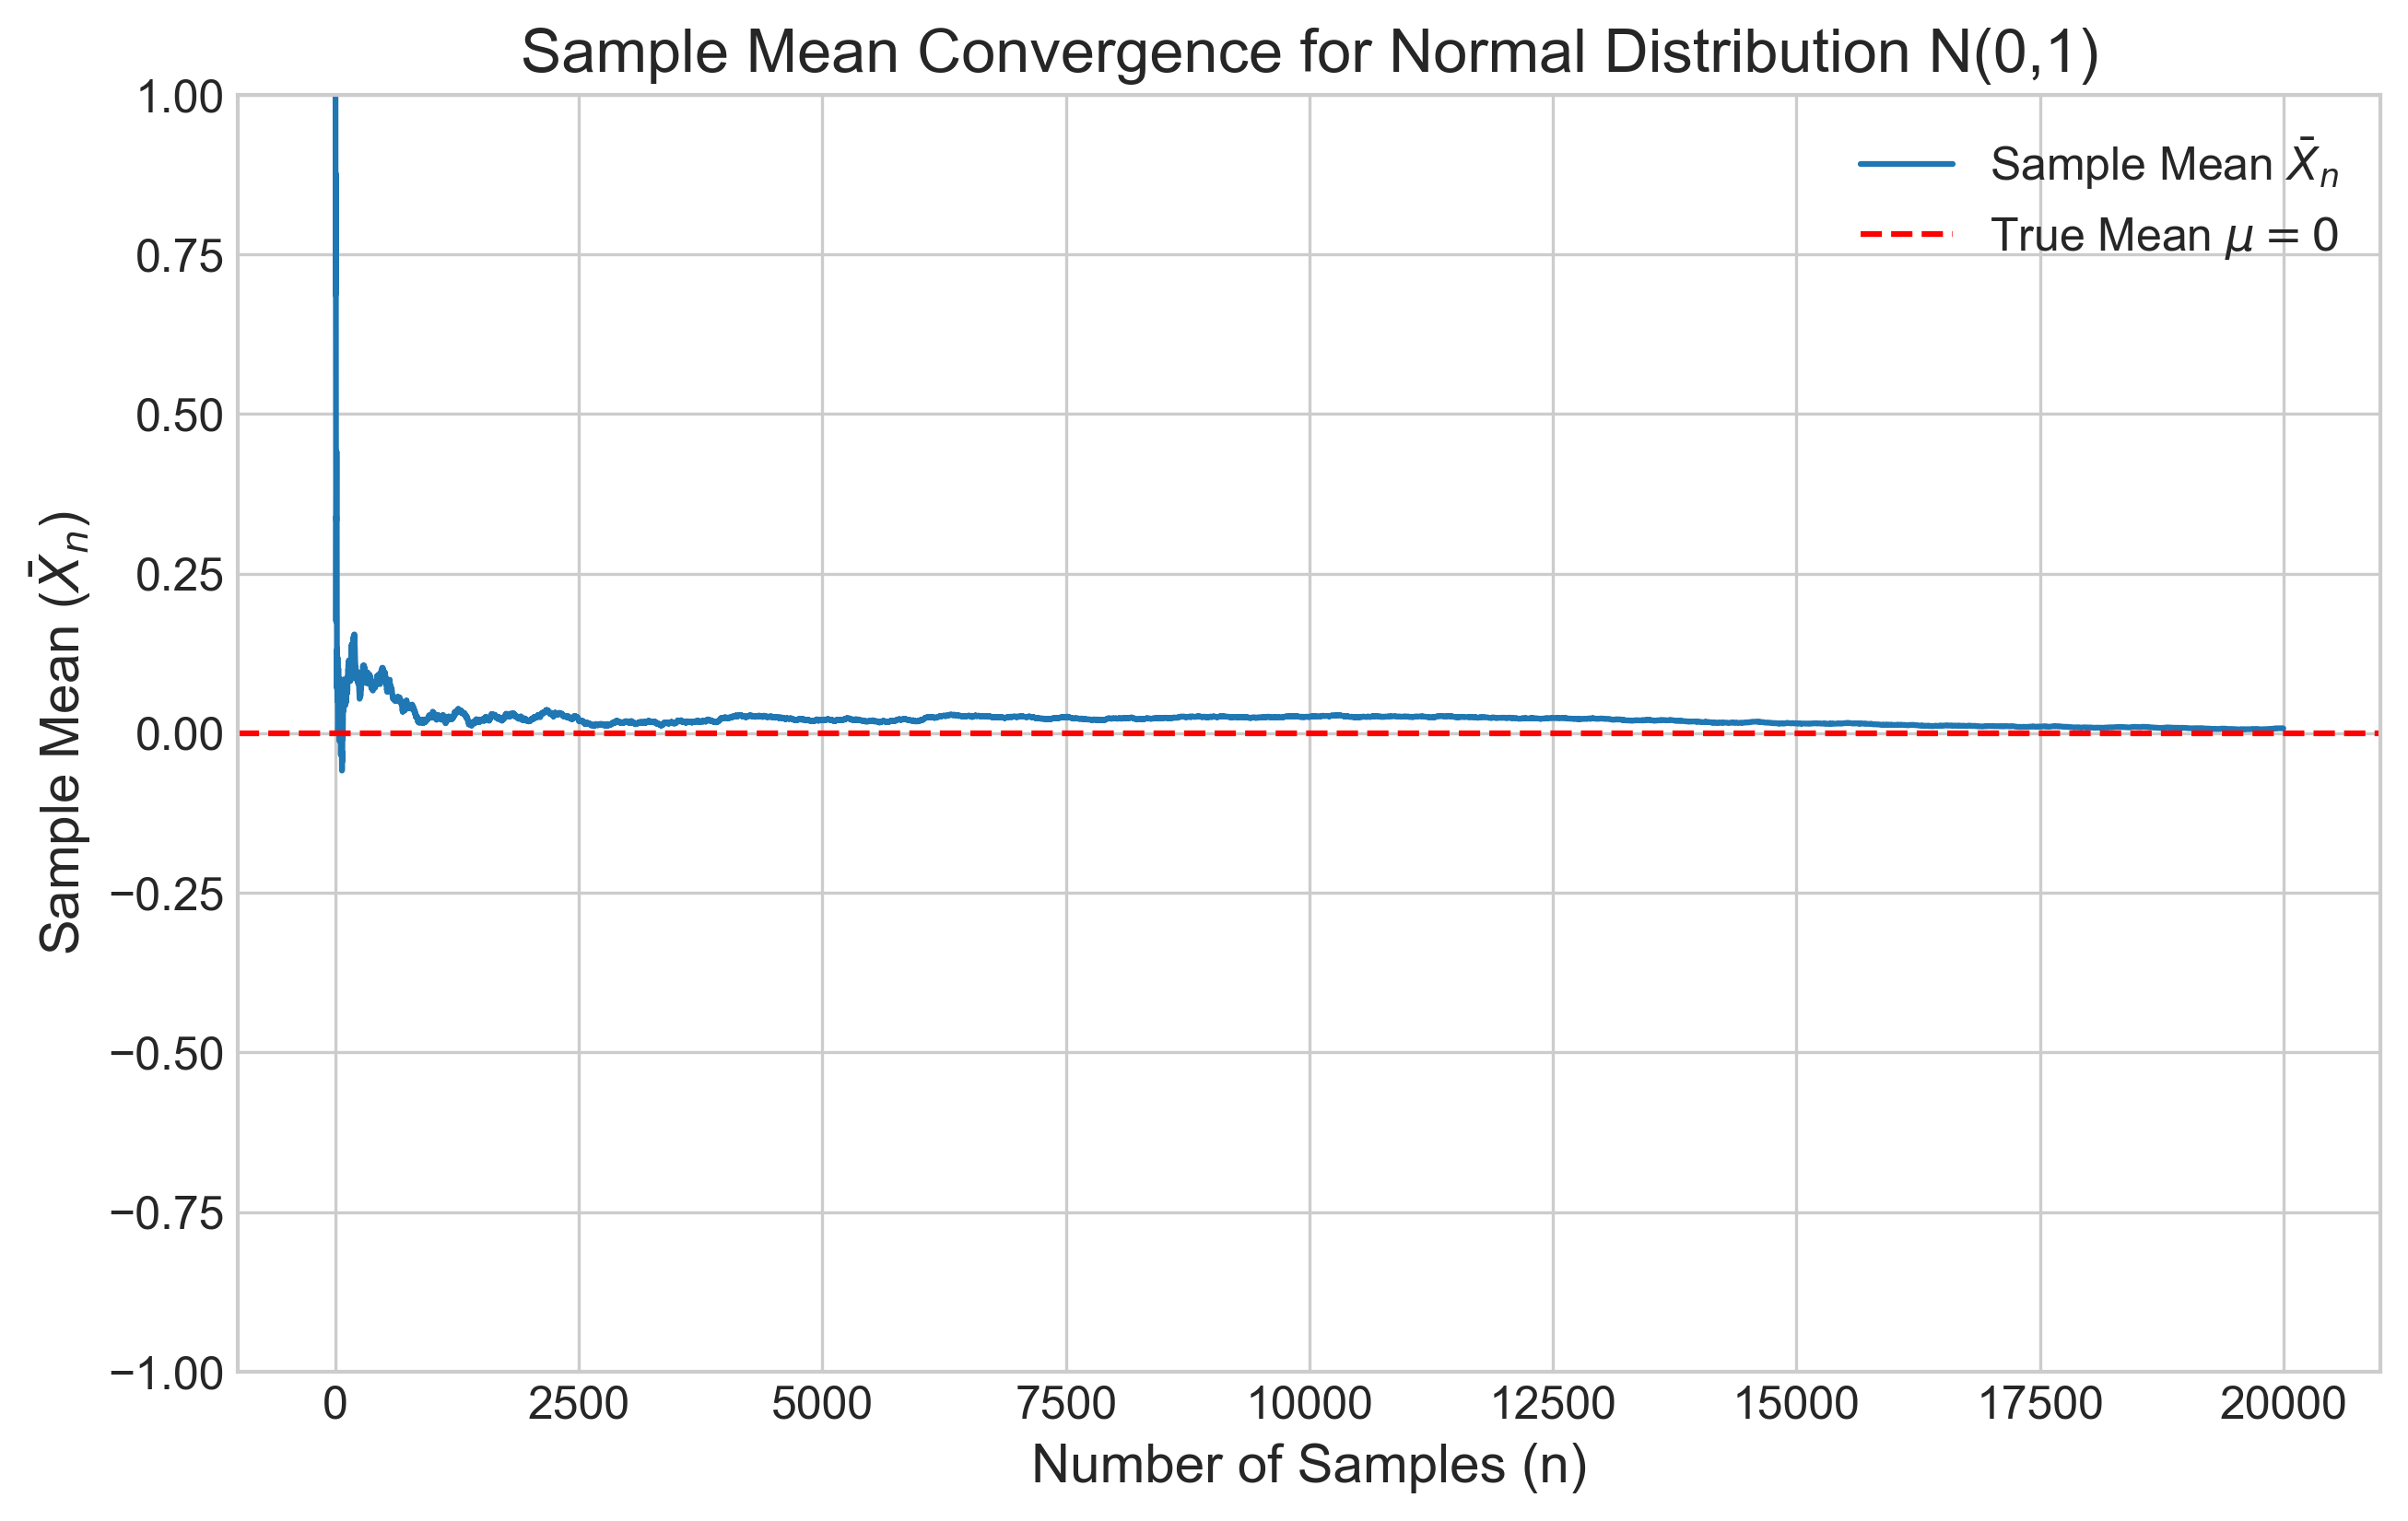
\includegraphics[width=\linewidth]{normal_mean_convergence.png} % REPLACE
                \caption{$\bar{X}_n$ 快速稳定收敛到 $\mu=0$}
            \end{figure}
        \end{column}
        \begin{column}{0.5\textwidth}
            \textbf{柯西分布 $C(0,1)$}\\($\E(X)$ 不存在)
            \begin{figure}
                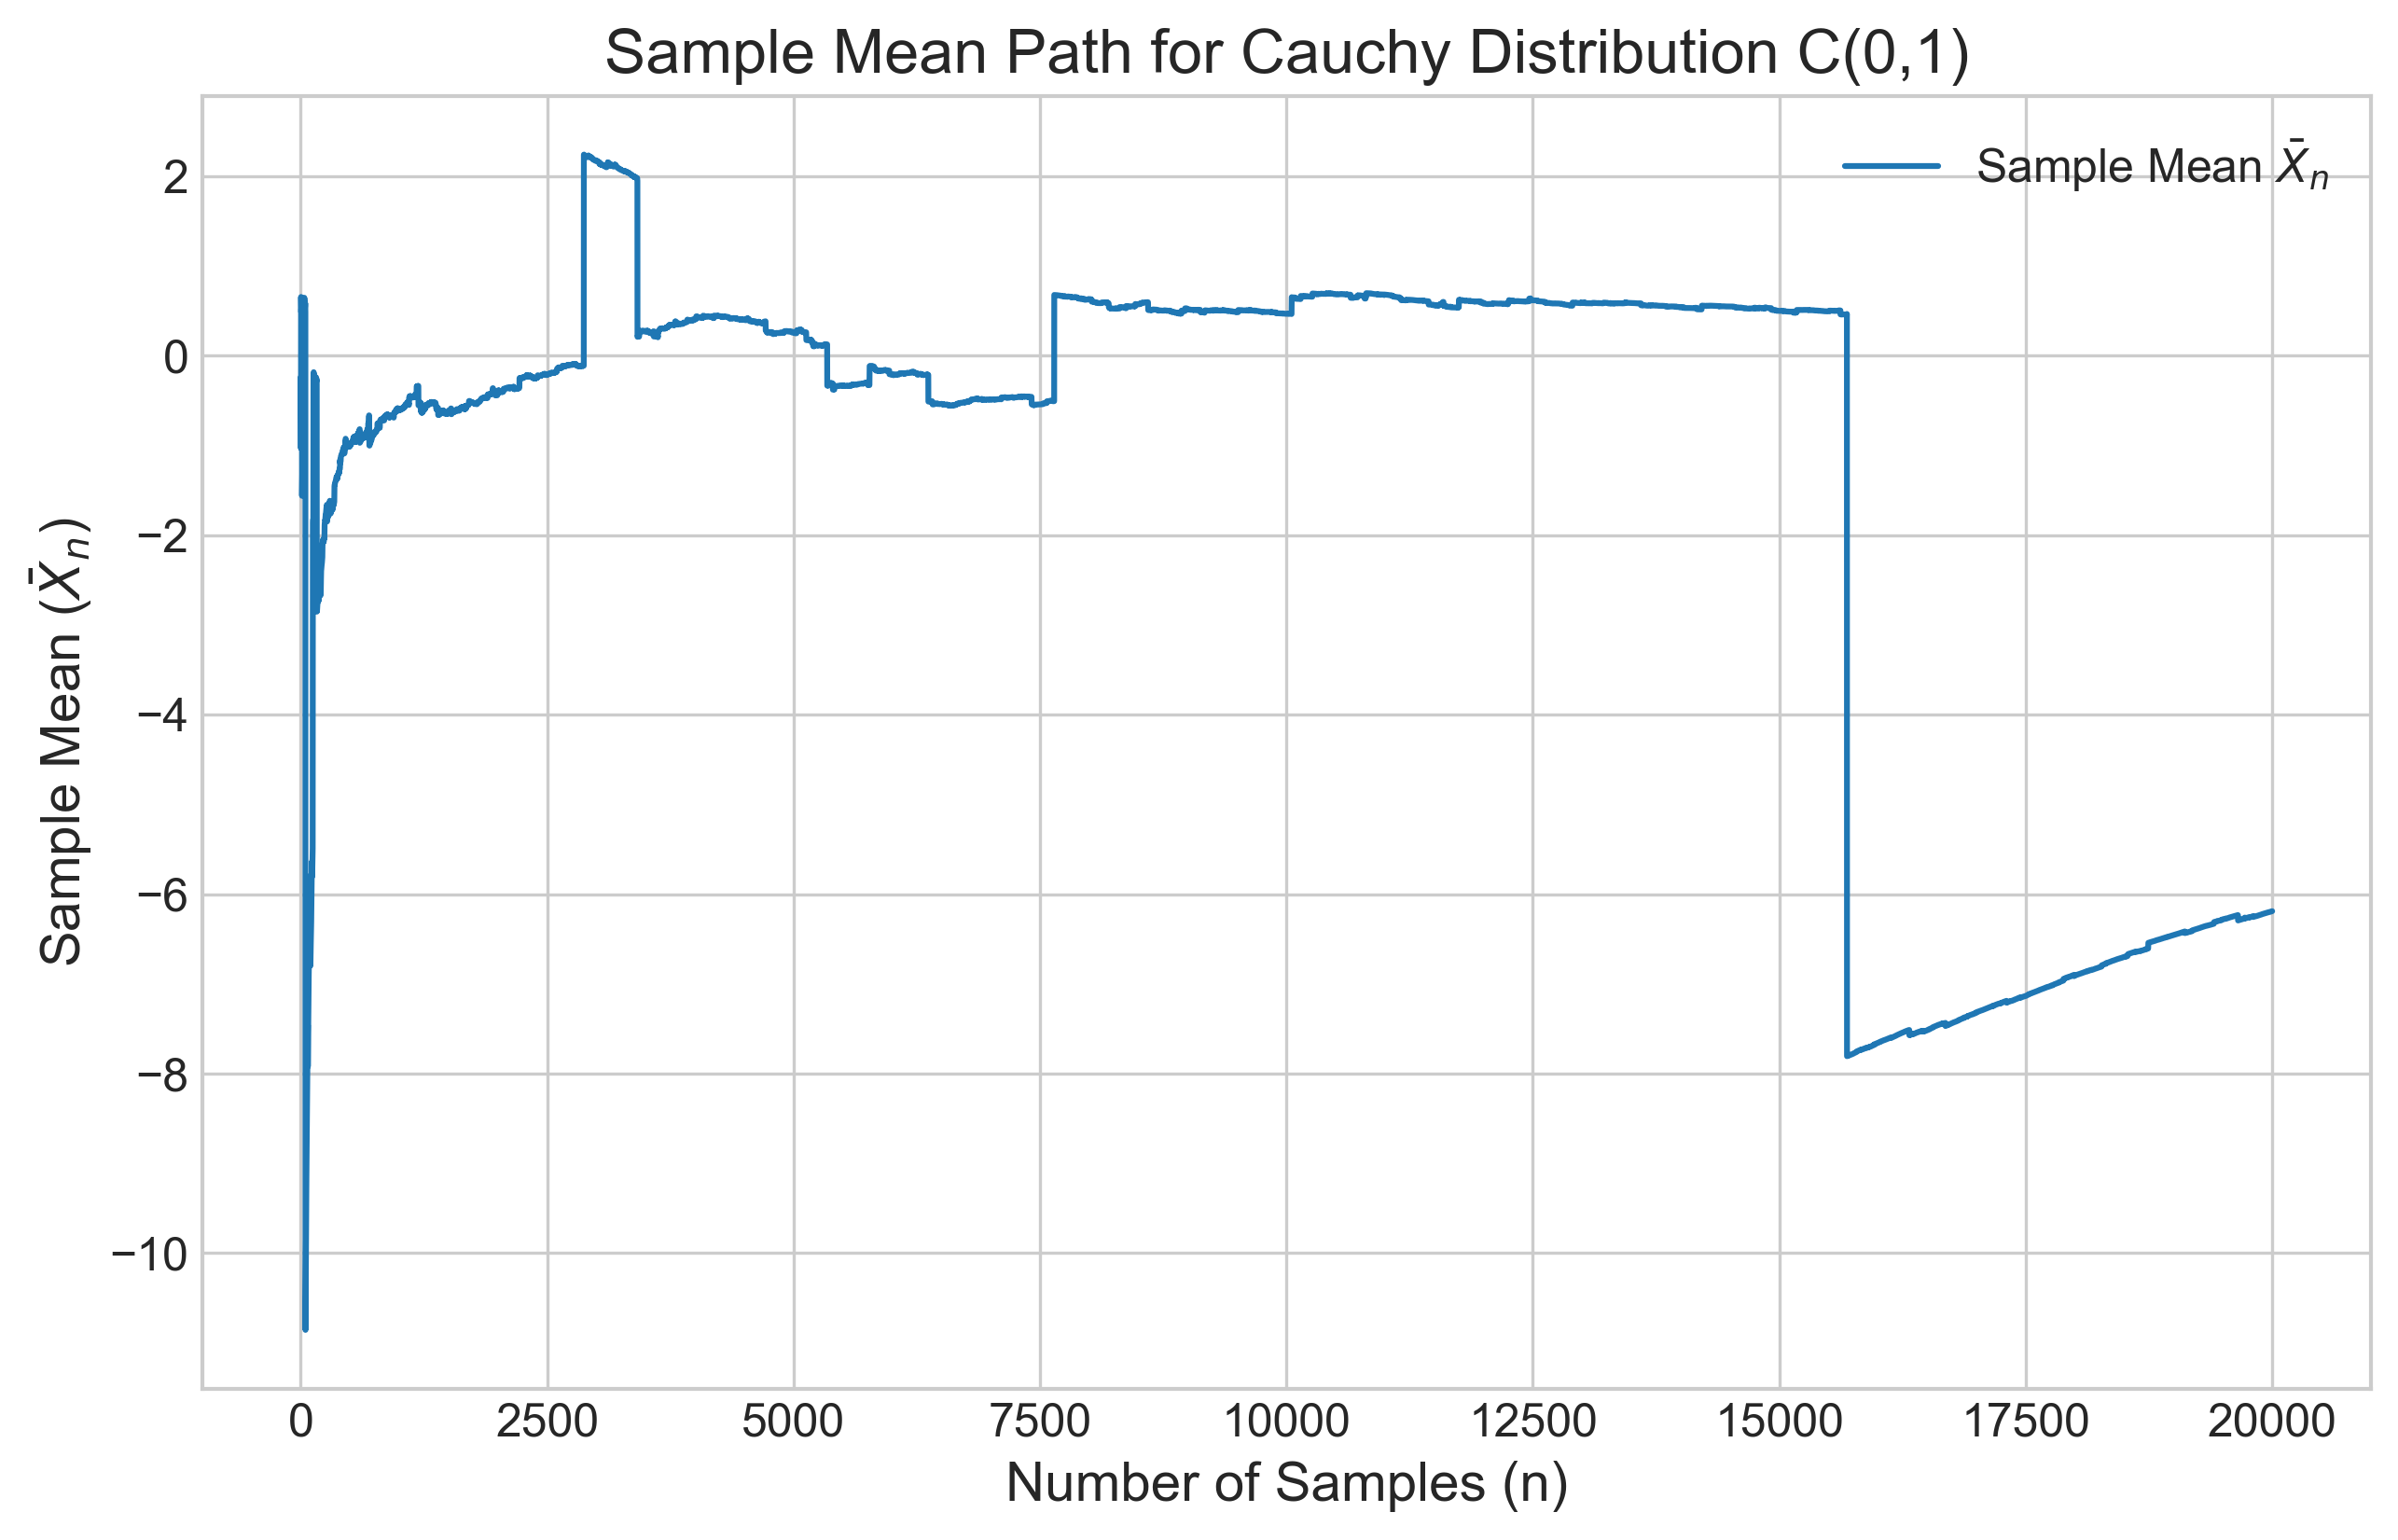
\includegraphics[width=\linewidth]{cauchy_mean_no_convergence.png} % REPLACE
                \caption{$\bar{X}_n$ 持续剧烈波动, \alert{不收敛}}
            \end{figure}
        \end{column}
    \end{columns}
    \textbf{启示}:
    \begin{itemize}
        \item 正态分布的样本均值行为良好,符合大数定律预期。
        \item 柯西分布的极端值持续"污染"样本均值,使其无法稳定。
    \end{itemize}
\end{frame}

\begin{frame}[shrink=10]{WLLN (续): 辛钦弱大数定律}
    \framesubtitle{期望存在即可 (i.i.d.情况)}
    \begin{block}{定理 7.4 (辛钦弱大数定律)}
        设 $X_1, X_2, \dots$ 是一列\alert{独立同分布 (i.i.d.)} 随机变量,其共同期望 $\E(X_i) = \mu$ \alert{存在} ($|\mu| < \infty$)。
        则样本均值 $\bar{X}_n = \frac{1}{n} \sum X_i \xrightarrow{P} \mu$。
    \end{block}
    \pause
    \textbf{对比应用:}
    \begin{itemize}
        \item \textbf{正态分布 $N(\mu, \sigma^2)$:}
            \begin{itemize}
                \item i.i.d.,期望 $\mu$ \alert{存在}。
                \item $\implies$ 满足辛钦WLLN条件,$\bar{X}_n \xrightarrow{P} \mu$。 (无需有限方差)
            \end{itemize}
        \item \textbf{柯西分布 $C(x_0, \gamma)$:}
            \begin{itemize}
                \item i.i.d.,但期望\alert{不存在}。
                \item $\implies$ \alert{不满足}辛钦WLLN条件,其结论不适用。
            \end{itemize}
    \end{itemize}
\end{frame}

\section{强大数定律 (SLLN)}
\begin{frame}[shrink=10]{7.3 强大数定律 (SLLN): 柯尔莫哥洛夫}
    \framesubtitle{更强的几乎必然收敛 (i.i.d.情况)}
    \begin{block}{定理 7.5 (柯尔莫哥洛夫强大数定律)}
        设 $X_1, X_2, \dots$ 是一列\alert{独立同分布 (i.i.d.)} 随机变量,其共同期望 $\E(X_i) = \mu$ \alert{存在} ($|\mu| < \infty$)。
        则样本均值 $\bar{X}_n = \frac{1}{n} \sum X_i \xrightarrow{a.s.} \mu$。
        ($\Prob(\lim_{n \to \infty} \bar{X}_n = \mu) = 1$)
    \end{block}
    \pause
    \textbf{对比应用:}
    \begin{itemize}
        \item \textbf{正态分布 $N(\mu, \sigma^2)$:}
            \begin{itemize}
                \item i.i.d.,期望 $\mu$ \alert{存在}。
                \item $\implies$ 满足柯尔莫哥洛夫SLLN条件,$\bar{X}_n \xrightarrow{a.s.} \mu$。 (结论更强)
            \end{itemize}
        \item \textbf{柯西分布 $C(x_0, \gamma)$:}
            \begin{itemize}
                \item i.i.d.,但期望\alert{不存在}。
                \item $\implies$ \alert{不满足}SLLN条件,其结论不适用。
            \end{itemize}
    \end{itemize}
    \footnotesize
    \textit{SLLN条件与辛钦WLLN相同 (i.i.d.且期望存在),但结论更强 (几乎必然收敛)。}
\end{frame}

\begin{frame}[shrink=5]{WLLN 与 SLLN 的区别与联系}
    \framesubtitle{依概率收敛 ($\xrightarrow{P}$) vs. 几乎必然收敛 ($\xrightarrow{a.s.}$)}
    \begin{columns}[T]
      \begin{column}{0.5\textwidth}
        \textbf{WLLN ($\xrightarrow{P}$)}:
        \begin{itemize}
            \item $\lim_{n \to \infty} \Prob(|\bar{X}_n - \mu| \geq \epsilon) = 0$
            \item 关注\alert{概率}:当$n$大时,$\bar{X}_n$偏离$\mu$很远的\alert{可能性}很小。
            \item 不排除在某些$n$处,$\bar{X}_n$可能偏离$\mu$较远,但这种事件发生的概率随$n$趋于0。
        \end{itemize}
      \end{column}
      \begin{column}{0.5\textwidth}
        \textbf{SLLN ($\xrightarrow{a.s.}$)}:
        \begin{itemize}
            \item $\Prob(\lim_{n \to \infty} \bar{X}_n = \mu) = 1$
            \item 关注\alert{样本路径}:对于\alert{几乎所有}的随机试验序列,$\bar{X}_n$的极限\alert{就是}$\mu$。
            \item 意味着除了一个概率为0的例外集合,$\bar{X}_n$最终会"停在"$\mu$处。
        \end{itemize}
      \end{column}
    \end{columns}
    \pause
    \textbf{强度与适用:} SLLN $\implies$ WLLN (几乎必然收敛更强)。
    \begin{itemize}
        \item \textbf{正态分布 $N(\mu, \sigma^2)$ (i.i.d.):} 期望 $\mu$ 存在。
            \begin{itemize}
                \item $\bar{X}_n \xrightarrow{P} \mu$ (由辛钦WLLN)
                \item $\bar{X}_n \xrightarrow{a.s.} \mu$ (由柯尔莫哥洛夫SLLN)
            \end{itemize}
        \item \textbf{柯西分布 $C(x_0, \gamma)$ (i.i.d.):} 期望不存在。
            \begin{itemize}
                \item $\bar{X}_n$ \alert{不}依概率收敛,也\alert{不}几乎必然收敛到任何常数。
                \item \alert{惊人事实}:若 $X_i \sim C(0,1)$ i.i.d.,则 $\bar{X}_n \sim C(0,1)$ 对所有$n$都成立!
            \end{itemize}
    \end{itemize}
\end{frame}

\section{大数定律的应用与警示}
\begin{frame}[shrink=5]{7.4 大数定律的应用与警示}
    \framesubtitle{理论指导实践,条件决定成败}
    大数定律是概率论与数理统计的重要基石:
    \begin{itemize}
        \item \textbf{频率稳定性}:为用频率近似概率提供了理论依据 (伯努利WLLN)。
        \item \textbf{参数估计}:样本均值 $\bar{X}_n$ 是总体期望 $\mu$ 的\alert{一致估计量}。
            \begin{itemize}
                \item \textit{例如:对于正态总体 $N(\mu, \sigma^2)$,用 $\bar{X}_n$ 估计 $\mu$ 是合理的。}
                \item \alert{警示}:\textit{若总体为柯西分布,$\bar{X}_n$ 不是其位置参数 $x_0$ 的一致估计量 (因 $\mu$ 不存在,LLN不适用)。用中位数估计 $x_0$ 更稳健。}
            \end{itemize}
        \item \textbf{蒙特卡洛方法}:通过大量随机抽样,用样本均值估计复杂积分或期望。
            \begin{itemize}
                \item \textit{适用于被积函数对应随机变量期望存在的情况。}
            \end{itemize}
        \item \textbf{风险管理与保险}:预测平均赔付,依赖于大量事件下平均损失的稳定性。
        \item \textbf{物理与工程}:多次测量的平均值通常比单次测量更接近真实值。
            \begin{itemize}
                \item \alert{警示}:\textit{如果测量误差服从柯西分布,增加测量次数并取平均\alert{无益于}提高精度!}
            \end{itemize}
    \end{itemize}
    \textbf{核心:大数定律的应用有效性,强依赖于其\alert{前提条件}(尤其是期望存在)是否满足。}
\end{frame}

\section{总结与展望}
\begin{frame}[shrink=10]{总结与展望}
    \begin{block}{本讲小结:大数定律的精髓与边界}
        \begin{itemize}
            \item \textbf{切比雪夫不等式}:提供了概率的通用上界(需期望、方差存在)。
            \item \textbf{大数定律}:描述样本均值在特定条件下收敛于总体期望。
                \begin{itemize}
                    \item WLLN (依概率 $\xrightarrow{P}$),SLLN (几乎必然 $\xrightarrow{a.s.}$)。SLLN更强。
                    \item 关键版本 (辛钦WLLN, 柯尔莫哥洛夫SLLN) 要求i.i.d.且\alert{期望存在}。
                \end{itemize}
            \item \textbf{正态分布 (i.i.d., $\E(X)=\mu$ 存在)}:
                \begin{itemize}
                    \item 样本均值 $\bar{X}_n \xrightarrow{P} \mu$ 且 $\bar{X}_n \xrightarrow{a.s.} \mu$。大数定律完美适用。
                \end{itemize}
            \item \textbf{柯西分布 (i.i.d., $\E(X)$ \alert{不存在})}:
                \begin{itemize}
                    \item 样本均值 $\bar{X}_n$ \alert{不收敛}。大数定律\alert{不适用}。
                    \item $\bar{X}_n$ 仍服从柯西分布,揭示了期望不存在时的特殊性。
                \end{itemize}
            \item 理解大数定律的\alert{条件和局限性}对正确应用至关重要。
        \end{itemize}
    \end{block}
    \pause
    \begin{alertblock}{展望:中心极限定理 (CLT)}
        \begin{itemize}
            \item 大数定律告诉我们样本均值\alert{收敛到哪里}。
            \item 下一步,\alert{中心极限定理 (CLT)} 将揭示:当 $n$ 很大时,样本均值围绕总体期望的\alert{波动形态}近似于何种分布 (通常是正态分布)。
            \item CLT 也有其前提条件,如经典的Lindeberg-Lévy CLT要求i.i.d.且具有\alert{有限的期望和方差}。这对正态分布适用,但对柯西分布 (因方差无限) 则不适用标准CLT。
        \end{itemize}
    \end{alertblock}
\end{frame}

\begin{frame}
    \centering
    \Huge{\bfseries 谢谢聆听!}
    \vspace{1cm}
    \normalsize
    问题与讨论
\end{frame}

\end{document}